\label{chap:04_hate_speech}

Los Discursos de odio contra mujeres, inmigrantes y muchos otros grupos es un fenómeno generalizado en la Internet. En los primeros días de la World Wide Web, algunos académicos se aventuraron a decir a que los prejuicios y el odio sería eliminado en este espacio por la disolución de identidades \cite{levy2001cyberculture, rheingold1993virtual}. Veinte años después de esta hipótesis, podemos
decir que no ha sido el caso. La prevalencia del racismo en la ``World White Web'' se ha estudiado en una serie de trabajos \cite{adams2005white, kettrey2014staking}, como así también la misoginia en el mundo virtual \cite{filipovic2007blogging, mantilla2013gendertrolling}.

El discurso racista y sexista es una constante en las redes sociales, pero los picos se documentan después de eventos ``detonantes'', como asesinatos con motivos religiosos o políticos \cite{burnap2015cyber}. Las empresas de redes sociales están preocupadas por esto y toman acciones en su contra; sin embargo, la mayoría de los esfuerzos todavía necesitan la intervención humana, lo que hace que esta tarea sea muy costosa. Reducir la intervención humana es vital para tener herramientas efectivas para evitar la escalada del discurso de odio.


En este capítulo haremos una introducción a este problema, que a su vez trataremos en los capítulos subsiguientes. Definiremos el discurso de odio y haremos una breve reseña de este fenómeno desde un marco legal y de tratados internacionales para luego centrarnos en este problema desde una perspectiva del procesamiento de lenguaje natural. En base al dataset de la competencia hatEval\cite{hateval2019semeval}, propondremos técnicas de detección de discurso de odio para las tareas propuestas, algunas de ellas presentadas en \citet{atalaya_tass2018}. Finalmente, marcaremos algunos problemas actuales en los enfoques actuales de la detección de discurso discriminatorio y algunas oportunidades de mejora que abordaremos en capítulos subsiguientes.


\section{Definición de discurso de odio}
\label{sec:hate_speech_definitions}

No existe una definición universalmente aceptada de lo que configura discurso de odio. Para intentar acercarnos lo más posible a este concepto, en esta sección haremos un repaso muy general de algunos tratados internacionales sobre la materia. Antes de continuar, hacemos \tbf{una aclaración:} en la normativa sobre derechos humanos muchas veces se encuentra delimitado el discurso \tbf{discriminatorio} del discurso de \tbf{odio}, siendo este último una subcategoría del primero de mayor intensidad y con incitaciones a la violencia contra grupos protegidos o individuos miembros de estos grupos. En la literatura de NLP sobre el tema se utiliza la expresión discurso de odio (\emph{hate speech}) para referirse indistintamente a ambos fenómenos.

Aún cuando entendemos que la acepción general del discurso de odio puede entenderse como incorrecta desde la perspectiva de tratados internacionales, teniendo en cuenta que esta tesis está centrada en técnicas para su detección automática usaremos esta terminología para plegarnos a los usos y costumbres de la comunidad de NLP.

\subsection{Abordaje desde una perspectiva legal y de los Derechos Humanos}

Un principio general que hace a los derechos más elementales del hombre y a la vida en sociedad es la posibilidad de expresarse libremente, el \tbf{derecho a la libre expresión}. Este derecho está protegido por constituciones nacionales y numerosos tratados internacionales. Uno de estos tratados, el Pacto Internacional de Derechos Civiles y Políticos (\emph{ICCPR} por sus siglas en inglés)\footnote{Este pacto desarrolla los derechos civiles y políticos establecidos por la Declaración Universal de los Derechos Humanos de la ONU}, sancionado en 1966 en la Asamblea de las Naciones Unidas y ratificado por 166 países, incluye en su artículo 19:

\begin{displayquote}[Artículo 19 de la ICCPR]
1. Nadie podrá ser molestado a causa de sus opiniones.

2. Toda persona tiene derecho a la libertad de expresión; este derecho comprende la libertad de buscar, recibir y difundir informaciones e ideas de toda índole, sin consideración de fronteras, ya sea oralmente, por escrito o en forma impresa o artística, o por cualquier otro procedimiento de su elección.

3. El ejercicio del derecho previsto en el párrafo 2 de este artículo entraña deberes y responsabilidades especiales. Por consiguiente, puede estar sujeto a ciertas restricciones, que deberán, sin embargo, estar expresamente fijadas por la ley y ser necesarias para:

a) Asegurar el respeto a los derechos o a la reputación de los demás;

b) La protección de la seguridad nacional, el orden público o la salud o la moral públicas.
\end{displayquote}

Este artículo que garantiza el derecho a la libertad de expresión da cuenta también de que esta libertad no es completamente irrestricta. El ejercicio de los derechos e igualdad ante la ley de otros marca este límite, no pudiéndose invocarse este derecho para avasallar los de terceros. La Convención Internacional sobre toda forma de Discriminación Racial (ICERD) \footnote{\url{http://servicios.infoleg.gob.ar/infolegInternet/anexos/120000-124999/122553/norma.htm}} dice en su artículo 4 al respecto:

\begin{displayquote}[Artículo 4, ICERD]

Los Estados partes condenan toda la propaganda y todas las organizaciones que se inspiren en ideas o teorías basadas en la superioridad de una raza o de un grupo de personas de un determinado color u origen étnico, o que pretendan justificar o promover el odio racial y la discriminación racial, cualquiera que sea su forma, y se comprometen a tomar medidas inmediatas y positivas destinadas a eliminar toda incitación a tal discriminación o actos de tal discriminación y, con ese fin, teniendo debidamente en cuenta los principios incorporados en la Declaración Universal de Derechos Humanos, así como los derechos expresamente enunciados en el artículo 5 de la presente Convención, tomarán, entre otras, las siguientes medidas:

a) Declararán como acto punible conforme a la ley, toda difusión de ideas basadas en la superioridad o en el odio racial, toda incitación a la discriminación racial así como todo acto de violencia o toda incitación a cometer tal efecto, contra cualquier raza o grupo de personas de otro color u origen étnico, y toda asistencia a las actividades racistas, incluida su financiación;

b) Declararán ilegales y prohibirán las organizaciones, así como las actividades organizadas de propaganda y toda otra actividad de propaganda, que promuevan la discriminación racial e inciten a ella y reconocerán que la participación en tales organizaciones o en tales actividades constituye un delito penado por la ley;

c) No permitirán que las autoridades ni las instituciones públicas nacionales o locales, promuevan la discriminación racial o inciten a ella.
\end{displayquote}


Los Estados y otros organismos deben entonces tomar medidas para poder asegurar el libre ejercicio de los derechos y la igualdad de todos sus miembros, aún cuando esto pueda significar una restricción en la libertad de expresión \cite{article192015}. Entendiendo entonces que este derecho tiene sus límites, podemos pensar que el discurso de odio es una de esas fronteras. Si bien este fenómeno es algo que no está completamente delimitado, repasaremos algunas definiciones de este fenómeno hechas en tratados para acercarnos un poco más a las características comunes que comparten las diferentes definiciones. La Observación General 35 del Comité por la Eliminación de la Discriminación Racial de la ONU (CERD) considera que será discurso de odio, y debe ser tipificado penalmente:

\begin{displayquote}[Recomendación 35 del Comité por la Eliminación de la Discriminación Racial, CERD]

    a) Toda difusión de ideas basada en la superioridad o en el odio racial o étnico, por cualquier medio;

    b) La incitación al odio, el desprecio o la discriminación contra los miembros de un grupo por motivos de su raza, color, linaje, u origen nacional o étnico;

    c) Las amenazas o la incitación a la violencia contra personas o grupos por los motivos señalados en el apartado anterior;

    d) La expresión de insultos, burlas o calumnias contra personas o grupos, o la justificación del odio, el desprecio o la discriminación por los motivos señalados en el apartado b) anterior, cuando constituyan claramente incitación al odio o a la discriminación;

    e) La participación en organizaciones y actividades que promuevan e inciten a la discriminación racial.
\end{displayquote}

%\citet{gagliardone2015countering} presenta un análisis de diversos organismos y sus definiciones de discurso de odio.

En líneas generales, como se menciona en el reporte de la CIDH sobre discurso de odio contra lesbianas, gay, trans e intersex en Latinoamérica \cite{CIDH2015}, el concepto usualmente es referido a expresiones que incitan a tomar algún tipo de medida hostil contra una víctima o un grupo de personas, siendo esta perteneciente a un determinado grupo social definido por alguna característica particular como ser la etnia, lenguaje, género, entre otras. Dicho esto, podría delimitarse el discurso discriminatorio del discurso de odio por la componente de la promoción e instigación de la violencia; sin embargo, para los fines de este trabajo utilizaremos los términos indistintamente. Aún cuando el discurso no contenga arengas ni incitaciones a cometer actos violentos, puede entenderse ese discurso como generador de un ambiente hostil y de intolerancia que termine promoviendo estos ataques físicos \cite{CIDH2015}.

\citet{article192015} condensa muchas de estas definiciones de una manera sucinta, desglosando esto en \textbf{odio} y \textbf{discurso}:

\begin{displayquote}[Article 19: Hate Speech Toolkit]
    1. Odio: emoción intensa e irracional de oprobio, enemistad y aborrecimiento hacia una persona o grupo de personas, por tener determinadas características protegidas (reconocidas en el derecho internacional), reales o percibidas. El “odio” es más que un mero prejuicio y debe ser discriminatorio. El odio es una muestra de un estado emocional u opinión y, por lo tanto, se diferencia de cualquier acto o acción que se haya llevado a cabo.
    2. Discurso: cualquier expresión que vierta opiniones o ideas, que comparte una opinión o una idea interna con un público externo. Puede adoptar muchas formas: escrita, no-verbal, visual o artística y puede ser difundida en los medios, incluyendo Internet, material impreso, radio o televisión.
\end{displayquote}

%%
%%
%% Link
%% https://docs.google.com/drawings/d/149dpb2nrvmFgWZJYcrToAxO4M5n7JNQInfWd62kw3jc/edit
%%
%%

\begin{figure}[t]
    \centering
    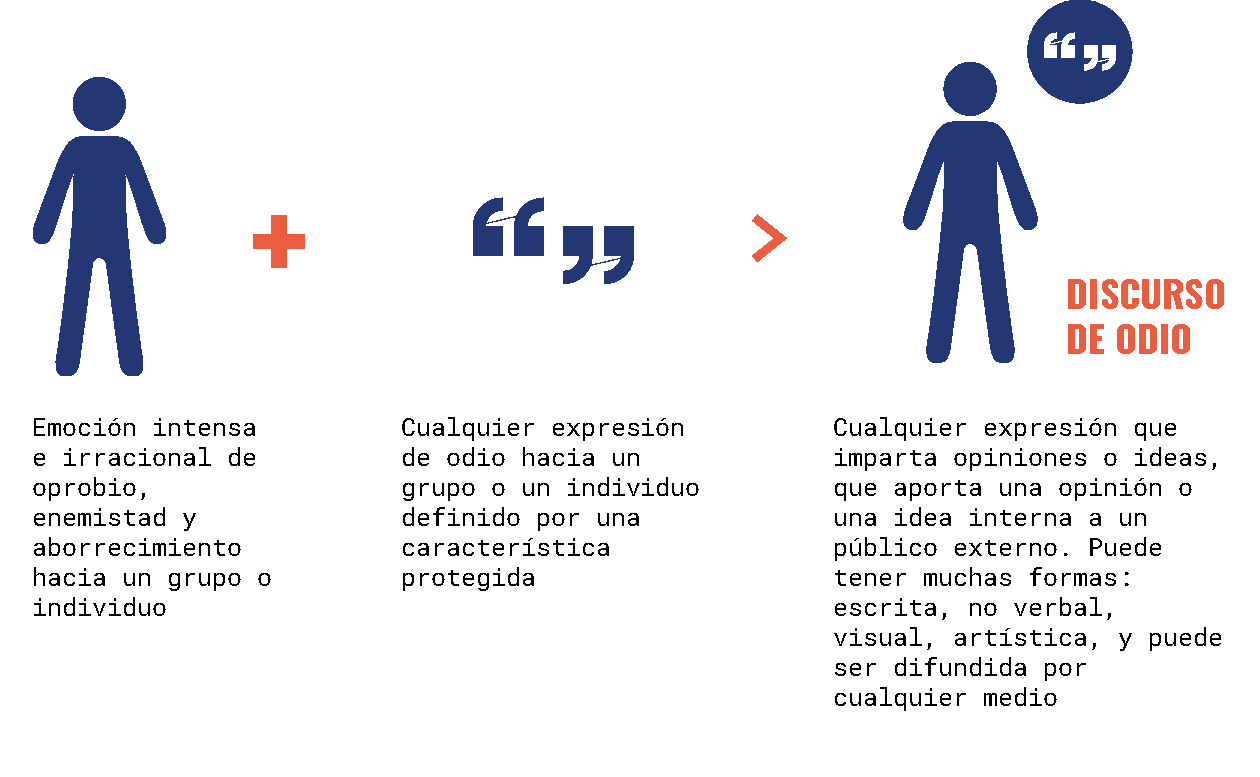
\includegraphics[width=\textwidth]{img/discurso_de_odio.pdf}
    \caption{Definición de discurso de odio de acuerdo al Toolkit de Article 19}
    \label{fig:hate_speech_definition_article_19}
\end{figure}


En base a esta definición, puede entenderse al discurso de odio como un discurso de cierta intensidad e irracionalidad que ataca a una persona o un grupo de personas por alguna característica históricamente vulnerada: por ser mujer, por su género, por su etnia, nacionalidad, religión, idioma, etc. La clave está en la combinación: un discurso irracional e intenso contra alguien que no posea una característica protegida no configura discurso de odio; por ejemplo, ataques a ciertas personas por ser periodistas. La figura \ref{fig:hate_speech_definition_article_19} ilustra esta definición.

No todo ataque a un individuo o una persona de algún colectivo discriminado es discurso de odio. En particular, la CIDH \cite{CIDH2015} menciona en base al informe de la UNESCO sobre discurso de odio \cite{gagliardone2015countering} que:

\begin{displayquote}[]
    (...) el discurso de odio no puede abarcar ideas amplias y abstractas, tales como las visiones e ideologías políticas, la fe o las creencias personales. Tampoco se refiere simplemente a un insulto, expresión injuriosa o provocadora respecto de una persona. Así definido, el discurso de odio puede ser manipulado fácilmente para abarcar expresiones que puedan ser consideradas ofensivas por otras personas, particularmente por quienes están en el poder, lo que conduce a la indebida aplicación de la ley para restringir las expresiones críticas y disidentes. Asimismo, el discurso de odio tiene que distinguirse de aquellos ``crímenes de odio'' que se basan en conductas expresivas, como las amenazas y la violencia sexual, y que se encuentran fuera de cualquier protección del derecho a la libertad de expresión
\end{displayquote}

Como vemos, no solamente es difusa la frontera fijada sobre qué es discurso de odio o insultos, sino que incluso también es difícil definir qué característica es protegida o no. En el siguiente capítulo hablaremos más de esto al describir los criterios utilizados a la hora de anotar un conjunto de datos sobre comentarios en Twitter.




\section{Trabajo previo}

En esta sección haremos una breve reseña de algunos trabajos destacados del área. Un análisis extensivo de esta disciplina escapa totalmente al alcance de este trabajo. Referimos a quien esté interesado a \citet{schmidt2017survey} y a \citet{fortuna2018survey}. Más recientemente, \citet{poletto2021resources} hace un análisis pormenorizado y actualizado de los recursos para la tarea de detección de discurso de odio.

La detección del discurso del odio es una tarea de clasificación de oraciones bastante relacionada con el análisis de sentimientos y ha sido estudiada para varias redes sociales \cite{thelwall2008social, pak2010twitter, saleem2017web}. Uno de los primeros trabajos al respecto es \citet{greevy2004classifying} usando bolsas de palabras y SMVs para detectar contenido racista en páginas web. Construyeron su dataset de manera semi-supervisada buscando sitios mediante keywords y sus links en motores de búsqueda. Siguiendo un enfoque similar, \citet{warner2012detecting} usó unigrams y clusters Brown con SVM para detectar mensajes antisemitas en Twitter.

\citet{waseem2016hateful} anotó un corpus y usó n-gramas de caracteres para detectar comentarios de odio, y \citet{badjatiya2017deep} usó el mismo conjunto de datos para entrenar modelos de aprendizaje profundo e incrustaciones ajustadas junto con Gradient Boosted Trees. \citet {zhang2018detecting} entrenó una red neuronal profunda que combina CNN con unidades recurrentes cerradas \cite{cho2014learning}, superando a los sistemas anteriores en varios conjuntos de datos.

\citet{anzovino2018automatic} recopiló un corpus de tweets misóginos y propuso una taxonomía para distinguirlos en diferentes categorías. Los autores propusieron una serie de técnicas diferentes para clasificarlos, mostrando que enfoques simples (como el uso de modelos lineales junto con n-gramas de token) logran un rendimiento competitivo en conjuntos de datos de pequeño tamaño.

En cuanto a las tareas compartidas, \citet{fersini2018overview} presentó un shared task en la detección de misoginia en Twitter, tanto en español como en inglés, mientras que \citet{fersini2018evalitaoverview} planteó un desafío similar pero en italiano e inglés. \citet{bosco2018overview} propuso un concurso de detección automática sobre publicaciones de Twitter y comentarios de Facebook, que incluía discursos de odio en general.



\section{Recursos}

En esta sección haremos un recuento de los conjuntos de datos para la detección de lenguaje odioso.
\citet{nobata2016abusive} fue uno de los primeros datasets => mencionar sus criterios, y su experimento (muy interesante) de Turkers vs anotadores in-house

% \begin{table*}
%     \centering
%     \begin{tabular*}

%     \end{tabular*}
% \end{table*}

\citet{gao2018detecting}

% \subsection{Criterios de anotación}

% \begin{table*}[t]
%     \centering
%     \begin{tabular}{p{0.20\linewidth}  p{0.80\linewidth}}
%         \textbf{Hate Speech} & Language which attacks or demeans a group based on race, ethnic origin, religion, disability, gender, age, disability,
%         or sexual orientation/gender identity. Some examples:
%         \begin{itemize}
%             \item The JEWZ are Market Manipulators Hate them freaking Jews !! To bad Hitler did not finish them off !!!
%             \item  I hate the mall because there are too many unemployed apefricans and mudsharks.
%             \item 300 missiles are cool! Love to see um launched into TelAviv! Kill all the gays there!
%             \item EGYPTIANS ARE DESCENDED FROM APES AND PIGS. NUKE EGYPT NOW Ah me tu se ku sh
%         \end{itemize} \\

%         \hline

%         \textbf{Derogatory} & Language which attacks an individual or a group, but which is not hate speech. Some examples:
%         \begin{itemize}
%             \item All you perverts (other than me) who posted today, needs to leave the O Board. Dfasdfdasfadfs
%             \item yikes...another republiCUNT weighs in....
%         \end{itemize} \\

%         \hline

%         \textbf{Profanity} & Language which contains sexual remarks or profanity. Some examples:

%         \begin{itemize}
%             \item T.Boone Pickens needs to take a minimum wage job in FL for a week. I guarantee he shuts the f up after that.
%             \item Somebody told me that Little Debbie likes to take it up the A.\$.\$.
%             \item So if the pre market is any indication Kind of like the bloody red tampons that you to suck on all day??
%         \end{itemize}
%          \\
%     \end{tabular}
%     \caption{Annotation guidelines used in \cite{nobata2016abusive}}

%     \label{tab:nobata_guidelines}
% \end{table*}

\todo{Mandar esto al siguiente capítulo}


\section{Dataset utilizado}




\begin{table}[t]
    \centering
    \small
    \begin{tabular}{l|l l l | l l l}
        Categoría  &    \mc{3}{Español}                          & \mc{3}{Inglés}                                \\
                   &    Train      & Dev          & Test         &    Train      & Dev          & Test           \\
        No HS      &2,643 (58.7\%) & 278 (55.6\%) & 940 (58.8\%) &5,217 (58.0\%) & 573 (57.3\%) & 1,740 (58.0\%) \\
        HS         &1,857 (41.3\%) & 222 (44.4\%) & 660 (41.2\%) &3,783 (42.0\%) & 427 (42.7\%) & 1,260 (42.0\%) \\
        TR         &1,129 (60.8\%) & 137 (61.7\%) & 423 (64.1\%) &1,341 (35.4\%) & 219 (51.3\%) & 529 (42.0\%)   \\
        AG         &1,502 (80.9\%) & 176 (79.3\%) & 474 (71.8\%) &1,559 (41.2\%) & 204 (47.8\%) & 594 (47.1\%)   \\
        Total      &4,500          & 500          & 1,600        &9,000          & 1,000        & 3,000          \\
    \end{tabular}
    \caption{Números del dataset de \citet{hateval2019semeval}, por idioma y por partición. No HS representa los tweets que no tienen contenido odioso, HS aquellos que sí, TR aquellos que son individualizados, y AG aquellos que son agresivos. Entre paréntesis encontramos los porcentajes de incidencia, considerando TR y AG dentro de aquellos que son discriminatorios}
    \label{tab:hateval_dataset}
\end{table}

El dataset que utilizamos en este capítulo es el provisto por \citet{hateval2019semeval}. Este dataset está orientado a la detección de discurso de odio contra mujeres e inmigrantes en Twitter, tanto en inglés como en español. Nuestro trabajo estará centrado en el dataset en español.

Posee las siguientes etiquetas:

\begin{itemize}
    \item \textbf{HS}: una etiqueta binaria que marca si el tweet tiene contenido discriminatorio (0 si no lo tiene, 1 si hay discurso de odio)
    \item \textbf{Target}: Si hay HS, una etiqueta binaria que marca si el objetivo del discurso de odio es un objetivo genérico (0) o si se refiere a un individuo específico (1)
    \item \textbf{Agresividad}: Si hay HS, una etiqueta binaria que marca si el tweet es agresivo
\end{itemize}


La tabla \ref{tab:hateval_dataset} posee los números del dataset. Podemos observar entre los dos idiomas que, si bien la proporción de discurso de odio se mantiene muy similar en ambos idiomas (58\% vs 42\% aproximadamente), la proporción de discurso de odio individualizado (TR) y agresivo (AG) es notoriamente más alto para el español. Esto puede deberse, entre otras cosas, a distintas estrategias de recolección de los datasets. La tabla ZZZ posee algunos ejemplos para cada una de las características en cuestión.

\section{Tareas de clasificación propuestas}

Sobre el dataset de hatEval, los autores propusieron dos tareas:

\newcommand{\subtaska}[0]{\textbf{Tarea A}}
\newcommand{\subtaskb}[0]{\textbf{Tarea B}}

\begin{itemize}
    \item \subtaska{}: Dado un tweet predecir si contiene discurso de odio contra mujeres o inmigrantes (HS)
    \item \subtaskb{}: Dado un tweet, predecir si contiene discurso de odio (HS), si está dirigido contra un individuo o un grupo (TR), y si es agresivo o no (AG)
\end{itemize}

\todo{Pensar algún nombre mejor?}

La primer tarea es la versión clásica de la detección de discurso de odio, donde predecimos una etiqueta binaria. La segunda es una versión más rica, de grano fino, donde predecimos varias características de particular interés para distinguir algunas formas potencialmente más peligrosas de este fenómeno.

La performance de \subtaska{} es medida mediante la Macro F1 de la clase positiva y negativa. En el caso de \subtaskb{}, se mide por la Macro F1 de las 3 clases (HS, TR, AG) y también por la medida Exact Match Ratio

\begin{equation*}
    EMR = \frac{1}{n} \sum\limits_{i=1}^{n} I(Y_i, Y_i^*)
\end{equation*}

siendo $Y_i$ las etiquetas respectivas $(HS, TR, AG)$, $Y_i^*$ las etiquetas que predice nuestro sistema, e  $I$ la función indicadora ($I(x, x) = 1$, $0$ en cualquier otro caso). Observado más de cerca, esto puede entenderse la accuracy sobre la 3-upla de la salida de los clasificadores, pero usamos la terminología de Exact Match Ratio como se usa en \citet{zhang-2014-multilabel} para referirse a esta métrica (a diferencia del Hamming Score).

\section{Método}

\subsection {Preprocesamiento}


\newcommand{\elmo}[0]{ELMo}
\newcommand{\elmomodel}[0]{\emph{LSTM-\elmo{}}}
\newcommand{\bow}[0]{BoW}
\newcommand{\boc}[0]{BoC}
\newcommand{\elmobowmodel}[0]{\emph{LSTM-\elmo{}+\bow{}}}
\newcommand{\svmmodel}[0]{$\mathrm{SVM}_0$}
\newcommand{\hateval}[0]{HatEval}
\newcommand{\semeval}[0]{SemEval-2019}
\newcommand{\fasttext}[0]{\emph{fastText}}

El preprocesamiento es crucial en las aplicaciones de PNL, especialmente cuando se trabaja con datos ruidosos generados por el usuario. Aquí, seguimos \citet{atalaya_tass2018}, definiendo dos niveles de preprocesamiento: preprocesamiento básico y orientado a sentimientos. Usamos uno u otro, dependiendo de la configuración.

El preprocesamiento básico de tweets incluye tokenización, reemplazo de identificadores, URL y correos electrónicos, y acortamiento de letras repetidas.

El preprocesamiento orientado a sentimientos incluye minúsculas, eliminación de puntuación, palabras vacías y números, lematización (usando TreeTagger \cite{schmid95}) y manejo de negación.
Para el manejo de la negación, seguimos un enfoque simple:
% \cite {das01, pang02}:
Buscamos palabras de negación y agregamos el prefijo 'NOT \_' a los siguientes tokens. Se niegan hasta tres tokens, o menos si se encuentra un token que no sea una palabra.

\section{Técnicas de clasificación}

Para capturar esta información, consideramos una representación de bolsa de caracteres que codifica recuentos de caracteres $n$ -gramas para algunos valores de $ n $. Estos vectores se calculan a partir de textos originales de tweets, sin ningún procesamiento previo. \boc {} s tienen las mismas variantes y parámetros que \bow {} s.


\subsection {Word-embeddings}

Usamos \fasttext{}, una biblioteca de embeddings basada en combinaciones lineales de sub n-gramas \cite{bojanowski16} para obtener representaciones de palabras independientes del contexto.


De la misma manera que en la anterior sección, en lugar de usar vectores previamente entrenados disponibles públicamente, entrenamos nuestras propias incrustaciones en un conjunto de datos de $ \sim90 $ millones de tweets de varios países de habla hispana.
Preparamos dos versiones de los datos: una usando solo preprocesamiento básico y la otra usando preprocesamiento orientado a sentimientos (con la excepción de la lematización). Para estos dos conjuntos de datos, las incrustaciones de omisión de gramática se entrenaron utilizando diferentes configuraciones de parámetros, incluyendo una serie de dimensiones, tamaño de n-gramas de palabras y subpalabras, y tamaño de la ventana de contexto.

\subsection{Tweet Embeddings}
\label{sec:sif}

%%
%%
%%
%%  https://docs.google.com/drawings/d/1BU3ulBiqU0NojpW6Fkb4xFlMCDigSWwfjN7z9smO6nY/edit
%%
%%

\begin{figure}[t]
    \centering
    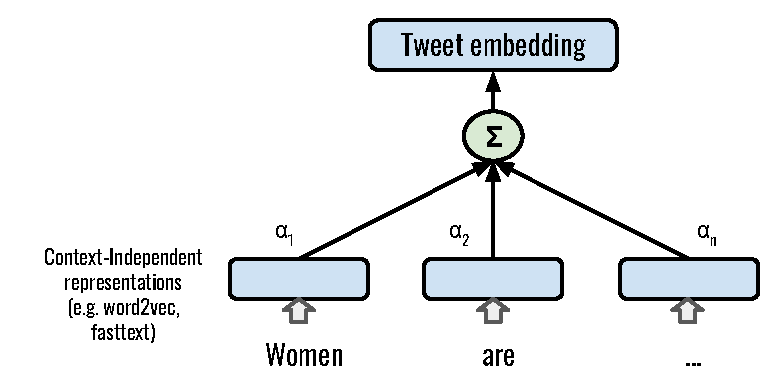
\includegraphics[width=\textwidth]{img/tweet_embeddings.pdf}
    \caption{Muestra de la recolección de datos}
    \label{fig:tweet_embeddings}
\end{figure}

Una forma relativamente simple de obtener una representación de una oración es realizar una combinación lineal de las representaciones obtenidas para cada palabra. Es decir, dada una oración $s = w_1 w_2 \ldots w_n$, y representaciones $\overline{w_1}, \overline{w_2}, \ldots, \overline{w_n} \in \mathbb{R}^m$, podemos obtener una representación

\begin{equation}
    \overline{s} = \sum\limits_{i=1}^{n} \alpha_i \overline{w_i}
\end{equation}

con $\alpha_1, \ldots, \alpha_n \in \mathbb{R}$ escalares (dependientes de la oración). De esta manera, obtenemos de $n$ representaciones independientes del contexto una representación para el tweet, sin tener en cuenta posibles interacciones entre los distintos componentes. La figura \ref{fig:tweet_embeddings} ilustra esta metodología simple para obtener representaciones de oraciones.

Tenemos entonces dos posibilidades para determinar la combinación lineal: la forma de obtener las representaciones, y la forma de calcular los coeficientes. Para las representaciones, podemos usar varias de las técnicas que ya vimos como word2vec, GloVe, o \fasttext{}. Para calcular los coeficientes, consideramos en nuestro trabajo dos formas. La primera, la forma canónica, calculando un promedio de las representaciones, es decir, tomando $\alpha_i = \frac{1}{n}$

Se utilizaron combinaciones lineales para calcular una representación de un solo tweet.
Seguimos dos enfoques simples: promedio simple y promedio ponderado. En el segundo caso, utilizamos un esquema que se asemeja a la frecuencia inversa suave (SIF) \cite {arora17}, inspirado en la reponderación de TF-IDF.
Cada palabra $ w $ se pondera con $ \frac {a} {a + p (w)} $, donde $ p (w) $ es la palabra probabilidad unigrama y $ a $ es un hiperparámetro de suavizado.
Los valores altos de $ a $ significan más suavizado hacia el promedio simple.

% También consideramos dos opciones que afectan las incrustaciones de tweets: binarización, que ignora las repeticiones de tokens en los tweets; y normalización, que escalas dando como resultado que los vectores de tweets tengan una norma unitaria.


\subsection{Embeddings contextualizados}
\label{subsec:elmo}

Después del gran salto adelante que representó las incrustaciones de palabras independientes del contexto, llegó una nueva ola en los últimos años. En lugar de tener vectores entrenados para cada palabra, se generan representaciones dependientes del contexto para cada token dada una oración. Por ejemplo, \citet{mccann2017learned} usó un codificador LSTM profundo para traducción automática para generar vectores sensibles al contexto.

\elmo{} \cite{peters2018} es uno de estos enfoques dependientes del contexto y se basa en un modelo de lenguaje bidireccional profundo (biLM). La arquitectura del modelo de lenguaje consta de L capas de LSTM bidireccionales, además de una representación de token independiente del contexto. Por lo tanto, para cada token en una secuencia, obtenemos representaciones vectoriales de $ 2L + 1 $.
% Estas representaciones se consideran profundas ya que utilizan la salida de cada capa LSTM.
Para obtener un vector final para cada token, los autores sugieren colapsar las capas en vectores mediante una combinación lineal.

% Sea $ t_1, \ldots, t_n $ una secuencia de tokens, y sea $ h_ {k, j} $ el vector que representa la salida de la capa $ j $ cuando se consume el token $ t_k $. Entonces, el vector contextualizado para el token $ k $ es:
%
% \begin {ecuación}
% ELMo_k ^ {tarea} = \gamma ^ {tarea} \sum_ {j = 0} ^ {L} s_j h_ {k, j} \label {eq: elmo}
% \end {ecuación}

En este trabajo, usamos la implementación y los modelos entrenados previamente de \cite{che-EtAl:2018:K18-2}. El modelo español se entrenó con $L = 2 $ capas y 1024 dimensiones, y la combinación lineal se realizó utilizando un promedio simple.

\subsection{Modelos}

Para las tareas propuestas, analizamos el desempeño de diversos modelos de clasificación. Algunos de ellos son los presentados para la shared-task \hateval{}, a las cuales agregamos modelos basados en transformers. Estos modelos no estaban disponibles al momento de presentar dicho trabajo. \footnote{El trabajo de BERT\cite{devlin2018bert} es de finales de 2018, y hasta finales de 2019 no fue publicada una versión entrenada en español, BETO}.

Para la tarea de detección binaria (\subtaska{}) planteamos 3 tipos de clasificadores:

\begin{itemize}
    \item Modelos lineales: regresiones logísticas y SVM con kernel lineales, consumiendo como entrada bolsas de palabras, bolsas de caracteres, y tweet embeddings usando SIF.
    \item Redes neuronales recurrentes: usando como entrada word-embeddings y embeddings contextualizados (\elmo{})
    \item BERT: Usamos la versión en español entrenada por \citet{canete2020spanish}, BETO.
\end{itemize}

Para el caso de la tarea de multidetección (\subtaskb{}), podemos pensar este problema de dos maneras:

\begin{enumerate}
    \item Un problema de clasificación múltiple
    \item Un problema de clasificación de 5 clases
\end{enumerate}

En el primer caso, el enfoque sería predecir por separado HS, AG, y TR. La segunda formulación se basa en observar que no todas las 8 combinaciones son permitidas, sino sólo 5: si no hay HS no nos interesa observar las otras dos variables. Tenemos entonces 5 clases a predecir.

Con esta última observación, propusimos en \citet{atalaya_tass2018} un modelo basado en SVM (consumiendo la misma entrada que detallamos anteriormente). No evaluamos en dicho trabajo un modelo recurrente con este esquema de clasificación, ni tampoco lo haremos aquí, considerando que evaluaremos modelos que han demostrado tener mejor performance para numerosas tareas de clasificación de texto.

\begin{figure}
    \centering
    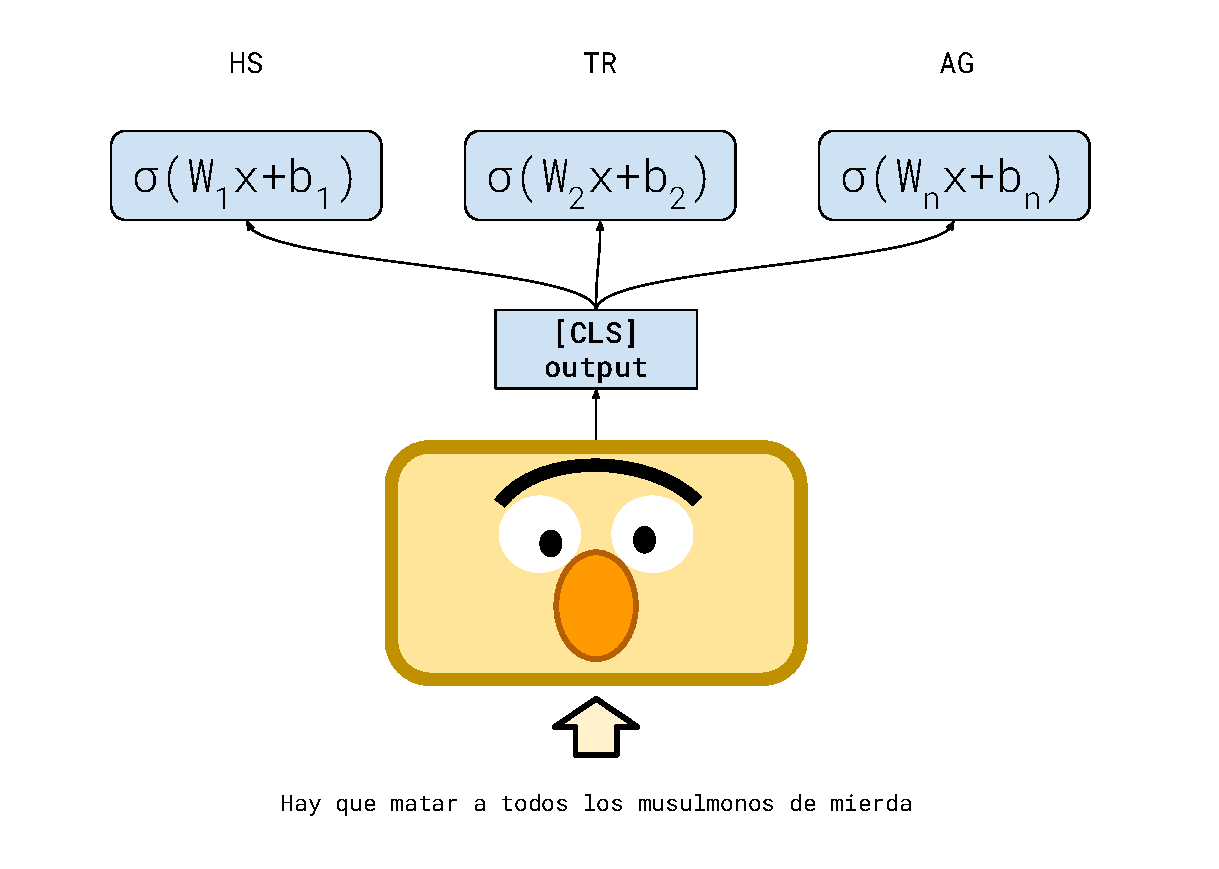
\includegraphics[width=\textwidth]{img/bert_model_hateval.pdf}
    \caption{Modelo basado en BERT para la tarea de clasificación múltiple}
    \label{fig:bert_hateval_classifier}
\end{figure}


Así mismo, proponemos para esta subtarea modelos basados en transformers basado en multi-clasificación. La arquitectura usual de modelos basados en BERT para clasificación constan de poner como última capa una  ``cabeza'' que consume la salida del token \verb|[CLS]|. En términos concretos, esto agrega una matriz de parámetros $W \in \mathbb{R}^{m \times 768}$ donde $m$ es la cantidad de clases de nuestro problema y 768 corresponde a la dimensión de cada vector del modelo de transformers, y usando softmax como función de activación.

Para construir un modelo de multi-clasificación, mantenemos la misma arquitectura pero, en lugar de usar como activación la función softmax, utilizamos la función sigmoidea elemento a elemento. En el caso de clasificación de $n$ clases, $softmax(W x + b)$ nos da para el elemento i-ésimo el score de que la instancia pertenezca a la clase $i$. Por otro lado, en el caso de multiclasificación de $n$ variables, $\sigma(W x + b)$ nos da el score de predecir la etiqueta positiva para el (en nuestro caso,  $\sigma(W x + b)_1$ nos da la probabilidad de que $HS = 1$,  $\sigma(W x + b)_2$ nos da la probabilidad de que $HS = 2$, etc). La figura \ref{fig:bert_hateval_classifier} ilustra el modelo utilizado.

Para entrenar el modelo de clasificación, evaluamos dos tipos de funciones de costo. En primer lugar, utilizamos la suma o promedio\footnote{Es equivalente optimizar una u otra} de las entropías cruzadas binarias. Concretamente, si $y = (y_{HS}, y_{TR}, y_{AG})$ son las etiquetas de una instancia e $\widehat{y}$ la predicción del modelo, la pérdida es:

\begin{equation}
\label{eq:multi_loss}
L(y, \widehat{y}) = \sum\limits_{k \in \{HS, TR, AG\}} J(y_k, \widehat{y_k})
\end{equation}

donde $J$ es la entropía cruzada. Esta función de pérdida, sin embargo, ignora cualquier tipo de jerarquía entre las variables; por ejemplo, si para una instancia tenemos $HS = 0$, toma la pérdida de las variables $TR$ y $AG$. Contemplamos entonces una variante de esta función para tener en cuenta esta jerarquía:

\begin{equation}
    \label{eq:hierarchical_loss}
    L(y, \widehat{y}) =  J(y_{HS}, \widehat{y_{HS}}) + \beta(y_{HS})\sum\limits_{k \in \{TR, AG\}} J(y_k, \widehat{y_k})
\end{equation}

donde $\beta(y_{HS})$ pondera la pérdida de las variables del segundo nivel de nuestra jerarquía. Una opción puede ser considerar $\beta(1) = 1, \beta(0) = 0$, donde ignoramos las pérdidas de las variables $TR, AG$ cuando no hay discurso discriminatorio. Análogamente, $\beta(y) = 1$ sería el caso descripto en la ecuación \ref{eq:multi_loss}.

Para generalizar esto, podemos agregar un hiperparámetro $\gamma \in [0, 1]$ para escribir $\beta(y) = (1-y) \gamma + y$.

Las evaluaciones de los modelos las realizamos poniendo una máscara por encima de estos modelos de clasificación múltiple de manera de evitar salidas incoherentes (por ejemplo, $HS = 0, TR = 1, AG= 0$).


\section{Resultados}
\newcommand{\esrow}[1]{\multirow{#1}{*}{es}}
\newcommand{\enrow}[1]{\multirow{#1}{*}{en}}
\newcommand{\tbf}[1]{\textbf{#1}}


\begin{table}

    \centering

    \begin{tabular}{l l| l l l}
        Modelo       & Idioma              & Recall     & Precision & Macro-F1 \\
        \hline
        SVM          & \mr{3}{es}          & Recall     & Precision & 0.730    \\
        ELMO-RNN     &                     & 0.753      & 0.669     & 0.735    \\
        BETO         &                     & 0.839      & 0.674     & 0.764    \\
        \hline
        ELMO-RNN     & \mr{4}{en}          & ?          & ?         & 0.471   \\
        BERT         &                     & 0.968      & 0.474     & 0.496   \\
        RoBERTa      &                     & 0.967      & 0.470     & 0.485   \\
        BERTweet     &                     & 0.958      & 0.495     & 0.546
    \end{tabular}
    \caption{Resultados de la evaluación para la detección de discurso de odio en datasets de desarrollo y test, medidas por la métrica macro F1. En negrita, el mejor resultado.}
    \label{tab:hateval_task_a}
\end{table}



La tabla \ref{tab:hateval_task_a} muestra los resultados de evaluación para los modelos propuestos para la detección de discurso de odio ``plana''. Marcamos con un asterisco aquellos modelos presentados en \citet{atalaya_tass2018}. Respecto a los resultados en español, podemos observar que entre los presentados para aquella competencia, el modelo basado en SVMs obtiene la mejor performance, aún contra aquel basado en embeddings contextualizados, obteniendo el mejor desempeño en dicha con $0.730$ de Macro F1. La pobre performance de ELMo contra un modelo mucho más simple puede deberse a un mal entrenamiento , y puede que también debido al cambio de dominio, contra los cuales la entrada de las SVM está mejor adaptada.

Para ambos idiomas, los modelos basados en transformers \cite{vaswani2017attention} obtienen la mejor performance, con considerables mejoras respecto a los modelos basados en ELMo (y a los SVMs en el caso del español). Particularmente, en el caso del inglés, BERTweet \cite{bertweet} obtiene la mejor Macro-F1. En el capítulo 7 presentaremos un modelo similar a BERTweet para español que mejora la performance sobre BETO, a la vez que evaluaremos sobre versiones de BETO ajustadas al dominio social\footnote{Un modelo que no evaluamos en el presente trabajo es la versión en español de RoBERTa, recientemente entrenada. En el capítulo 7 evaluaremos su performance}.

La tabla \ref{tab:hateval_task_b} muestra los resultados de la \subtaskb{}, reportado por las F1 de cada variable predicha (HS, TR, AG), así como por el Macro F1 de HS y el Macro F1 de las 3 variables mencionadas. Los resultados están expresados como la media de 10 corridas independientes del experimento para cada configuración distinta. Consideramos las 3 versiones: Multi refiere a clasificación múltiple, Jerárquica a clasificación múltiple con la función de costo jerárquica, y Combinatoria a la conversión del problema en una clasificación de 5 clases.

Podemos observar que para español, la mejor performance en términos de EMR (la métrica más estricta) es el clasificador entrenada con la función de costo definida en \ref{eq:hierarchical_loss} (con el hiperparámetro $\gamma = 0.1$); sin embargo, esta diferencia la diferencia entre las performances no es significativa al correr un test de Kruskal-Wallis ($H(9) = 3.492, p = 0.174$). En términos de Macro-F1, la mejor performance es de BETO con el problema de clasificación múltiple y sin la función de costo jerárquica, pero de nuevo esta diferencia no es significativa ($H(9) = 3.656, p=0.16$).

Respecto al inglés, los mejores resultados pueden observarse en el modelo entrenado con BERTweet con la salida de 5 clases. Este resultado, sin embargo, queda en términos de EMR por debajo del baseline, y contemplando el Macro F1 de los mejores resultados de la competencia, obtenidos por el equipo MITRE \cite{gertner-etal-2019-mitre}. En ese trabajo se basaron en un ensemble de modelos entrenados con BERT, usando también un ajuste de dominio sobre tweets. Esta baja performance de nuestros modelos (y de los modelos en general sobre ese dataset) puede deberse a problemas de anotación y de que las particiones de train y test no son idénticamente distribuid

Algo que puede observarse es que, lejos de dañarse la performance de la detección de lenguaje discriminatorio (lo que analizamos en la \subtaska{}), predecir varias variables pareciera mejorar la performance. Este resultado puede verse en ambos idiomas, obteniendo cerca de (+1 puntos de Macro F1, y cerca de +4 puntos Macro F1 en inglés). \todo{Correr un test estadístico para ver si esto es significativo}.



\begin{table}
    \small
    \centering
    \begin{tabular}{lll rrr rrr}
        Modelo            & Salida         & Idioma     &  HS F1     & TR F1        &  AG F1        &   EMR       &  Macro F1       & Macro HS F1 \\
        \mr{3}{beto}      & multi         & \mr{3}{es}  &  0.741     &  \tbf{0.765} &  \tbf{0.688}  & 0.685       &     \tbf{0.731} &  0.771      \\
                          & jerárquico    &             &  0.735     &  0.758       &  0.674        & \tbf{0.703} &     0.722       &  0.776      \\
                          & combinatoria  &             &  \tbf{742} &  0.763       &  0.668        & 0.698       &     0.724       &  0.776      \\

        \hline
        \mr{3}{BERT}      & multi         & \mr{3}{en}  &  0.638     &  0.600       &  0.443        & 0.380       &     0.560       &  0.512      \\
                          & jerárquico    &             &  0.642     &  0.592       &  0.451        & 0.388       &     0.562       &  0.521      \\
                          & combinatoria  &             &  0.644     &  0.593       &  0.442        & 0.398       &     0.560       &  0.531      \\
        \mr{3}{BERTweet}  & multi         &\mr{3}{en}   &  0.658     &  0.629       &  0.462        & 0.426       &     0.583       &  0.567      \\
                          & jerárquico    &             &  0.656     &  0.617       &  0.450        & 0.423       &     0.574       &  0.555      \\
                          & combinatoria  &             &  0.666     &  0.637       &  0.444        & 0.449       &     0.582       &  0.589      \\
    \end{tabular}

    \caption{Resultados de la evaluación para la detección de discurso múltiple de discurso de odio, \subtaskb{}, en términos de las F1 de las clases HS (Hate Speech), TR (Targeted), AG (Aggressive), el Exact Match Ratio (EMR), las Macro F1 de las clases en cuestión, y la Macro F1 de la clase HS.  }
    \label{tab:hateval_task_b}
\end{table}




\subsection{Análisis de Error}
\label{sec:hateval_error_analysis}

\begin{figure}[t]
    \centering
    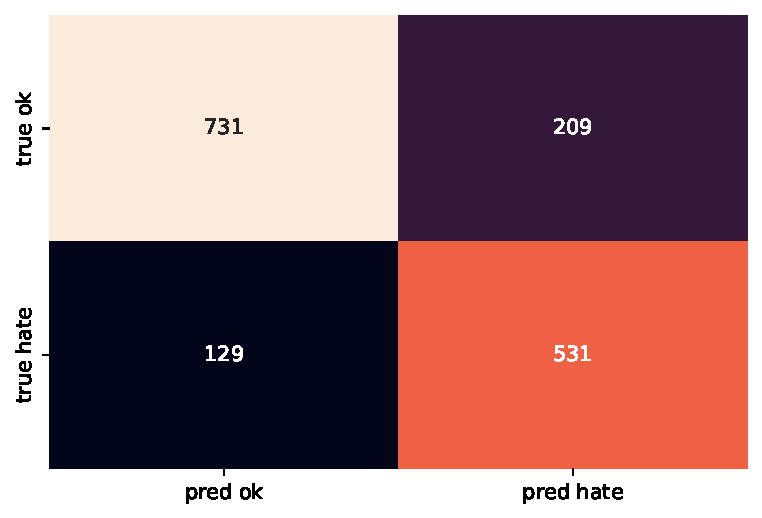
\includegraphics[width=0.6\textwidth]{img/hateval_confusion_matrix.pdf}
    \caption{Error analysis of the model}
    \label{fig:hateval_error_analysis}
\end{figure}


Para tener una mejor idea de lo ocurrido con nuestros clasificadores, realizamos un análisis de error sobre los datasets en español. Para intentar mitigar los efectos de la varianza de los clasificadores, tomamos las salidas de 10 clasificadores BETO entrenados con una distinta semilla y analizamos el error sobre un clasificador de ensamble por voto mayoritario; de esta manera, tratamos de buscar aquellos errores frecuentes, aquellos que la mayoría de los 10 clasificadores erran. Nos centraremos en observar los errores de la etiqueta HS, y particularmente veremos qué pasa con los falsos positivos. La figura \ref{fig:hateval_error_analysis} muestra la matriz de confusión de nuestros clasificadores. Como era de esperar (dado que la precisión es más baja que la sensitividad) tenemos muchos falsos positivos, por lo cual haremos eje en observar estos errores.


\begin{table}
    \begin{tabularx}{\columnwidth}{l X}
        Índice   &  Tweet \\
        \hline
        1   & Una cosa que le pasó a una amiga mexicana en Barcelona. Una chica repartía flyers en castellano y catalán, le dio uno a mí amiga en catalán y al segundo se lo quitó y se lo dio en castellano. -No, déjalo que entiendo catalán -Ah, es que como te he visto cara de sudaca Racismo 0 URL \\
        2   & Los fascistas salen de la ratonera para atacar a los 100 inmigrantes que han logrado saltar la valla de Ceuta. Asco de prensa y partidos políticos que se pelean por lograr los votos de los fascistas. Ningún ser humano es ilegal. \\
        3   & @saludhernandezm Esas personas que extrañan dictaduras, cualquier dictadura, aún más si son las ibéricas que ponen como eje a Madrid; su cultura, política e idioma sobre la idiosincrasia de los demás. Esos mismos que añoran a Franco y viven en un país 'Sudaca' creyéndose dueños de la verdad.	 \\
        4   & @caciena después sigo siendo un sudaca pero bueno \\
        5   & @ArturoMonteduro Pues tienes toda la razón del mundo. Y lo peor es que seguro que tenía papeles y DNI español, pero queda mejor decir "argelino" o "uno d'estos del top manta", "puto inmigrante", o "moro mierda" y ya pues matas dos pájaros de un tiro. \\
        6   & Obvio me ofendo cuando algn Sudaca hace algn comentario presuponiendo que los mexicanos somos feos, o que el pas est de la verga. Entre mexicanos podemos hablar mierda de Mxico, pero que a ningn pinche extranjero se le ocurra, porque va a haber pedo! \\
        7   & TODOS LOS INMIGRANTES Y GITANOS FUERA!!! Menos: el colombiano que me vende coca, el negro que me consigue putas, el moro que me pasa costo y el gitano que me vende maría. \\
        8   & Ayer nos fuimos a tomar algo con los cumpas: Dos españoles, un ponja, un africano y un sudaca. Estamos para campaña de United Colours of Benneton. \\
        \hline
    \end{tabularx}

    \caption{Falsos positivos del modelo de clasificación para la detección de discurso de odio (HS).}
    \label{tab:hateval_error_analysis}
\end{table}


En la tabla \ref{tab:hateval_error_analysis} podemos observar algunos de los errores que comete nuestros clasificador. Por un lado, podemos observar que algunos errores se deben a cierto overfitting a ciertas palabras ``clave'' (como las nro. 1, 2 y 3) muchas de las cuales son producto del proceso de recolección que está fuertemente basada en keywords (inmigrante, sudaca, por ejemplo). Haciendo un poco de probing en los clasificadores, podemos ver que ciertas palabras como ``sudaca'' o ``migrante'' automáticamente disparan una salida odiosa \footnote{Puede probarse esto en el cuadro interactivo de \url{https://huggingface.co/pysentimiento/robertuito-hate-speech?text=migrante}. Si bien este modelo es el que presentaremos en el capítulo \ref{chap:07_domain_adaptation}, la idea se mantiene}. Otros de los casos que nuestros clasificadores no parecieran detectar son los reportes de discriminación (como el caso 5, parcialmente también el 1) o casos de apropiación cultural (caso 3 o 5) o contenido irónico (casos 3, 4, 7 y 8 ). Estos casos dan cuenta de la dificultad de la detección de esta tarea.

Así mismo, en el proceso del análisis de error descubrimos algunos tweets a los cuales pareciera faltar contexto para poder tomar una decisión. Si bien esto a veces puede ser inferido por un humano (por ejemplo, infiriendo que un comentario habla de tal o cual suceso), un clasificador necesitaría esa información. Para el dataset en concreto, muchos de estos comentarios tienen un contexto implícito: muchos tweets hablan de incidentes en la frontera de Ceuta (España) entre inmigrantes y la policía, debido al proceso de recolección realizado. La tabla \ref{tab:hateval_lack_of_context} muestra algunos de estos ejemplos.



\begin{table}
    \begin{tabularx}{\textwidth}{l X}
        Etiqueta      & Tweet \\
        \hline
        \mr{13}{No HS} & - @ArturoMonteduro Pues tienes toda la razón del mundo. Y lo peor es que seguro que tenía papeles y DNI español, pero queda mejor decir ``argelino'' o ``uno d'estos del top manta'', ``puto inmigrante'', o ``moro mierda'' y ya pues matas dos pájaros de un tiro.      \\
                      & @UbedaJoseA @WalkingDead\_AMC Perro cállate ala puta       \\
                      & @iancandado Es sudaca como.tu       \\
                      & @Stopfalsasdenun Pero que tienes en la cabesaaaa?(con voz de sudaca de mierda)       \\
                      & @\_Lassana\_ Me la has puesto como un tanque apuntando a un campanario negrata		       \\
                      & @odiomistweets Es una analogía pendejo sudaca	       \\
                      & @MifasolMaite Sudaca? K racista eres \\
                      & @ElQuemaMarias te parece que un sudaca tatuado excelentemente bien dotado y carismático no es buen ejemplo?       \\
                      & @HQGatica @AnglicaVillarN1 Este sueco con cara de bolita .xq eso es este aspiracional desclasado . x dignidad debería irse . no lo hará xq este sudaca no la tiene !!!       \\
                      & @SOFIAGAVIRIAC Ambas cosas y Sudaca (lo que eso signifique)       \\
                      & @SleeplessXenn @envdiaN Este finde te recojo y vamos al barrio negrata de envdian       \\
                      & @elmundoes El q quería quitar concertinas y luego quitarse a los inmigrantes !!       \\
                      & @AlexTor1975 @sanchezcastejon Disfràcese de moro o negro, y al momento tiene resuelto el problema de espera, de verdad, mano de santo!. Nada como ser invasor, refugiado, o inmigrante en este paraíso terrenal. Ahora, si eres nativo del paraíso!!!!, Se te puede complicar la existencia!!!!. \\
        \hline
        \mr{2}{HS}    & CALLATE YA Y HAZME LA PUTA CENA JODERRR URL \\
                      & Basta ya de buenismo, si te no respetas a la polica ni a la guardia civil en la frontera nada de concertinas, simplemente 4 tiros. Fin del problema \\
                      & @benemeritosGC La solución es fácil, muro de hormigón de 3 metros de alto, garitas cerradas para vigilancia y por delante la valla actual con concertinas. No es caro, es cuestión de quererlo hacer. \\
                      & Por desgracia, no queda otra, aportan poco y nos cuestan mucho. Incluido nuestra seguridad. \#Inmigración \#Immigration URL \\
        \hline
    \end{tabularx}
    \caption{Algunos ejemplos observados en el análisis de error que carecen de contexto conversacional.}
    \label{tab:hateval_lack_of_context}
\end{table}


Algo que observamos también es que hay una fuerte cantidad de errores de etiquetado. La tabla \ref{tab:hateval_label_errors} muestra algunos de estos ejemplos. Si bien es difícil establecer una causa específica para cada uno de estos errores, es posible que sean causados por una combinación de: confusión entre lenguaje ofensivo y discurso de odio; un mismatch cultural entre los anotadores; falta de contexto; algunos tweets que fueron mal recolectados

\begin{table}
    \begin{tabularx}{\textwidth}{l X}
        Etiqueta      & Tweet \\
        \hline
        \mr{13}{HS} &Callate la puta boca pesada @Lauu\_tb \\
           & me cansada tía cállate ya la puta boca lo que te queda de vid \\
           & FLOR SALTANDO AHÍ LA RE PUTA MADRE TE LO MERECES PEDAZO DE FORRA TE LO MERECES, EN LA CARA DE TODOS HIJA ASÍ SE HACE \\
           & Callate! cerra el orto un ratooo! es mas, no te queres morir mejor? la puta que te pario  \\
           & @csdb530 @carvasar Claro, porque la culpa la tienen las niñas embarazadas y las víctimas de acoso sexual, violación… https://t.co/f16xSqT37G \\
           & @nlopezi\_ Imbécil tu puta prima! Gilipollas! Estúpida \\
           & Esta mujer es lo más la puta madre https://t.co/8SWPhKbXQe \\
           & \#Pendejos Don't call me gringo You fuckin beaner Stay on your side Of that goddamn river Don't call me gringo You beaner No me digas beaner Mr. puñetero Te sacaré un susto Por racista y culero No me llames frijolero Pinche gringo puñetero \\
           & Mónica que te calles la puta boca \#OTGala7 \\
           & @bastadetopos Callate que me camine dosmillonesquinientas cuadras para llegar el semi. La puta que los parió a todos. \\
           & @pablocasado\_ @imbrodamelilla @TeoGarciaEgea pablo no quieren concertinas , un muro de 12 metros o mas de altura de dos plantas de pisos ,se acabo los problemas @guardiacivil @policia @EMADmde @MonarquiaEspana nadie se quejaría de nada \\
           & \#OTGala7 Noemí JAJAJAJAJAJA ESTA MUJER ES LA PUTA AMA \\
           & No puedo creer lo que le hicieron a Cersei, yo se que es una hija de puta pero ni así se merecia lo que le hicieron… https://t.co/uftkVl5ene \\
        \hline
    \end{tabularx}
    \caption{Ejemplos mal etiquetados}
\end{table}


\todo{Esto falta}

\section{Discusión}

Respecto a lo relativo a la performance de los modelos presentados, los modelos basados en transformers son notoriamente superiores a los demás modelos. Particularmente, en inglés, podemos observar que aquellos directamentre pre-entrenados sobre tweets (BERTweet) tienen mejor performance que aquellos que son pre-entrenados sobre wikipedia como BERT o RoBERTa.

Sobre la tarea más difícil de detección múltiple de discurso de odio (\subtaskb{}), propusimos varios enfoques: uno basado en predecir cada variable por separado y otro en predecir una variable que indique la combinación en cuestión. El modelo de predicción múltiple entrenado con la función de costo jerárquica \ref{eq:hierarchical_loss} obtuvo la mejor performance, sin embargo, estas diferencias no se mostraron significativas. En el caso de inglés, el modelo entrenado sobre 5 clases obtuvo la mejor performance; sin embargo, esta dista de la mejor performance de la competencia. No ahondaremos en un análisis de estos resultados en inglés debido a los posibles problemas de anotación del dataset, y porque estamos más interesados en profundizar sobre la creación de recursos en español.

Algo que merece cierta atención es que, lejos de empeorar el desempeño de nuestros modelos, agregar nuevas variables a predecir (además de la existencia de discurso de odio) pareciera mejorar levemente la performance de la detección de este fenómeno, a la vez que obteniendo salidas más ricas e interpretables. \citet{gertner-etal-2019-mitre} exploró modelar las variables latentes de la característica ofendida, con alguna mejora en su performance\todo{chequear esto}. Teniendo esto en cuenta, podría uno preguntarse si contar con esta información (la o las características agredidas) se puede mejorar la performance de los clasificadores o tener salidas más interpretables que sólo una etiqueta binaria.

Hacemos a continuación una disquisición no sólo sobre este trabajo y el dataset en el que se basa sino en líneas generales sobre los recursos y enfoques actuales en el área de detección de discurso de odio. Continuando con la idea del párrafo anterior, una limitación que puede verse es que la mayoría de los trabajos atacan una, dos, o a como mucho tres características protegidas. Por ejemplo, los datasets de \cite{waseem2016hateful} y \cite{hateval2019semeval} (el utilizado en esta tarea) sólo consideran racismo y sexismo, mientras que \citet{Davidson2017AutomatedHS} agrega homofobia a esta consideración. Sería deseable poder contar con un dataset que como mínimo cuente con estas tres características en conjunto a otras quizás menos utilizadas: odio de clase (a veces conocida como ``aporofobia''), discriminación por aspecto físico, o por discapacidad. Esto, desde ya, con un framework unificado de anotación y no recolectando datasets anotados individualmente.

Un problema particular que se puede observar en este dataset (pero que atraviesa a muchos otros) es el proceso de recolección de los datos: los tweets son recolectados mayormente a través de keywords. Como está explicado en el overview de esta shared-task \cite{hateval2019semeval}, se usó para su recolección una combinación de estrategias. Sin embargo (ver sección XXX), hay una altísima incidencia de algunas palabras (como \emph{sudaca} o \emph{inmigrante}) que sesgan fuertemente el dataset. Esto (entre otras cuestiones) puede ser un problema para los modelos que se entrenan sobre estos datos, haciendo que aprendan correlaciones espurias. Si bien pueden aplicarse técnicas de regularización (como \emph{data augmentation}) para mitigar
esto, no deja de ser un problema. De todas formas, esto es una limitación general para estos tipos de aprendizaje sobre datos crudos y etiquetas, donde es difícil establecer e interpretar cómo un clasificador termina encontrando patrones para detectar el fenómeno medido.

La \textbf{anotación}, la etapa subsiguiente a la recolección de datos, pareciera presentar en este dataset algunos problemas. Hemos visto en la anterior sección una lista no extensiva de numerosos errores de etiquetado, aún cuando este dataset fue realizado con un etiquetado de 2 + desempate. Si bien es difícil trazar las razones detrás de estos problemas, observando las instancias podría uno imaginarse que esto es producto de un no entendimiento de las expresiones en los distintos dialectos del español. \citet{waseem-2016-racist} mostró que las anotaciones ``amateurs'' (producto del uso de crowdsourcing) tienden a tener mayores instancias de Hate Speech (algo que daría la impresión de ocurrir aquí) y que datasets anotados por expertos mejoran la performance de los modelos. Este problema podría profundizarse dado que no queda claro si los anotadores son hablantes nativos de español.

%%
%% Falta de contexto
%%

Un problema que observamos en el dataset estudiado en este capítulo (pero que aplica a otros también) es la \textbf{falta de contexto}: muchos de los mensajes carecen de información adicional sobre la noticia o el tema del que se está hablando. Cuando leemos un mensaje de un tweet, casi siempre los leemos en el contexto de una noticia, o un trending topic. Muy rara vez leemos un mensaje en total aislamiento. De hecho, gran parte de los comentarios de este dataset tiene un contexto implícito: la noticia de conflicto migratorio en Ceuta. Otros comentarios, por otro lado, no se entienden bien ya que son respuestas a un tweet y que según el hilo de conversación pueden entenderse o no como discriminatorios.

Un género no explorado en estos mensajes (usualmente aislados) son aquellos en los cuales el contexto es necesario para extraer un significado. Por ejemplo, un comentario que dice ``hay que matarlos'' puede o no entenderse como discurso de odio. Si el objeto del mensaje se refiere a mosquitos, ese mensaje no es odioso; si, por otro lado, está hablando sobre chinos en el contexto del COVID-19, entonces ese mensaje es discriminatorio (y además llama a tomar una medida violenta). En ese sentido, podemos preguntarnos sobre este punto es si el acceso a información contextual nos puede auxiliar en la detección de discurso de odio. Por ejemplo, tener acceso a una noticia, al hilo de conversación

Así mismo, otro problema que suele ocurrir relacionado al anterior es que no tenemos \textbf{información granular} de los datos anotados. Si bien algunos trabajos agregan información de la característica vulnerada, la mayoría simplemente agrega una etiqueta binaria sobre la existencia o no de discurso de odio (o bien algún nivel intermedio como si hay o no discurso ofensivo, como el caso de \citet{Davidson2017AutomatedHS}). Teniendo en cuenta lo observado en este capítulo, agregar información más detallada sobre cada caso puede ayudar a mejorar la detección del discurso de odio mediante una señal más rica a nuestros clasificadores sobre las diferentes fronteras de cada característica.

\subsection{Interpretabilidad y fragilidad de clasificadores}

\todo{Ver si esto va o es muy tirado de los pelos ya que es un problema más general de AI}

\section{Conclusiones}

En este capítulo hemos hecho una primer acercamiento a la tarea de detección de lenguaje discriminatorio, haciendo un repaso de su definición desde una perspectiva legal y social\todo{?}, así como también desde una perspectiva técnica analizando técnicas de clasificación usando el dataset presentado en la shared task multilingual \emph{hatEval}\cite{hateval2019semeval}. En base a este dataset, analizamos dos tareas: detección binaria de discurso de odio, y detección de múltiples variables (si es discurso de odio, si es dirigido, si es agresivo).

Para estas tareas, presentamos varios modelos de clasificación. Por un lado, clasificadores lineales que consumen distintos tipos de entrada como ser tweet embeddings y bolsas de caracteres; modelos recurrentes que consumen embeddings contextualizados; y finalmente, modelos del estado del arte basados en modelos de lenguaje pre-entrenados usando la arquitectura de transformers. Para ambas, los modelos de transformers

En el caso de la tarea de detección múltiple, propusimos dos formas de atacar el problema: como clasificación múltiple (prediciendo simultáneamente las 3 variables), y convirtiendo a un problema de clasificación simple sobre 5 clases posibles. Observamos, a su vez, que lejos de dañar la performance de la detección de discurso de odio, predecir más de una variable mejora la performance de nuestros clasificadores.

Analizando este dataset y algunos otros de la bibliografía, marcamos algunas puntos de mejora en la detección de discurso de odio: principalmente, la falta de información contextual. La mayoría de los datasets no tienen mayor información sobre los mensajes de los usuarios, algo que usualmente no pasa en las redes sociales. Por otro lado, y teniendo en cuenta la observación hecha en el párrafo anterior, nos preguntamos si tener información más granular acerca de las características . Finalmente, observamos que para la creación de datasets de un fenómeno tan complejo y social es indispensable tener muchos recaudos a la hora de la anotación, algo que ya ha sido observado en otros trabajos \todo{Citar trabajo sobre la performance de entrenar sobre datos de crowdsource vs etiquetadores especializados}.

En los siguientes capítulos, exploraremos algunas de estas observaciones. Particularmente, nos centraremos en la incorporación de contexto en la detección de discurso discriminatorio, construyendo un dataset que incorpore esta información a los mensajes anotados. Luego de eso, abordaremos la pregunta ¿puede el contexto de un mensaje ayudar a mejorar la detección de discurso de odio?